The Physics Office GitLab project aims to simplify the ATLAS documents (papers, CONF-Notes, internal notes...) creation, editing and publication process by using the tools provided by the CERN GitLab system. The usual publication workflow consisted on a heavy e-mail communication between ATLAS editors and Physics Office in order to ensure that ATLAS rules were beeing followed before being able to submit the desired paper to arXiv or to the journal of choice. This approach lead, usually, to modifications done in different sides (Officers and editors) not properly implemented by the other side which slows down the process due to small details which with a different approach would be easily fixeable.

There are three main areas modified by the PO-GitLab approach with the goal of simplifying this process. These areas are the automatic creation of the document GitLab projects (git repositories in a centralized way), the real-time check by the GitLab Continuous Integration (CI) tools of the documents being written and the automatic processing of the document to ensure a smooth publication process. These areas are descrived in detail in this section.

\subsection{Automatic document creation}
First, a centralized area controlled by ATLAS Physics Office needs to be dessigned. The control is key in order to allow Physics Office to maintain quality controls over the document being accepted for publication. The ATLAS Physics Office GitLab group (Described in \Sect{\ref{sec:pogitlab-group}}) has been created. This GitLab group (a set of users, subgroups and projects) hosts the git repositories of ATLAS Physics Office tools as well as subgroups, one for each physics group as defined in Glance.

Since there is a centralized and standardize place to host and maintain the document repositories, these are created automatically for each analysis group once they are created in Glance in the Analysis interface. This means that the creation of configuration of the repositories holding the document is done without any input from the editor's side allowing for a quick process.

\subsection{Real-time check with GitLab's CI}
GitLab CI tools are dessigned to execute a set of automatic tasks everytime a new modification is introduced in the document (i.e. a new commit is pushed to the document repository). These tasks can be as complicated as needed within the limits of the system. The approach from Physics Office was to develop a package which is able to run different jobs on a given document checking different aspecs. This is the \texttt{pogitlab} python package~\cite{pogitlab-repo}

GitLab's CI works in Pipelines; each a time a new commit is pushed to the repository a pipeline is triggered. A pipeline is a set of jobs grouped in stages. All the jobs in the same stage are run in parallel while each stage is only executed once the previous one has finished. The real-time checks are run in most of the branches of the project, lets call them \epipes. The \epipes, showing an example in \Fig{\ref{fig:edit-pipe}} consist in the following set of stages:

\begin{itemize}
  \item \textbf{Preparation:} It consist of only one job which checks that the current version of the \texttt{pogitlab} package.
  \item \textbf{Technical checks:} This stage includes checks related to \LaTeX\:
  \begin{itemize}
    \item \textit{Figures exist:} check if all figures used throughout the document are present in the repository or if anyone is missing.
    \item \textit{Files exist:} check if all the \textit{.tex} files included in the document are present~\footnote{The files and figures exist checks are needed because it is rather common to forget committing a new file or figure.}
    \item \textit{Repeteated commands:} checks for repeated user defined commands. It is not wise to use the same command for different purposes and can be an issue when generating captions for figures and tables for the ATLAS public pages.
    \item \textit{Repeated labels:} checks for duplicated labels all documents.
    \item \textit{Undefined references:} checks for undefined references.
    \item \textit{Unused labels:} warnings against label which has been defined but not used. Although this is not an issue it might point to something not being properly referenced.
  \end{itemize}
  \item \textbf{ATLAS checks:} These are checks related to ATLAS rules and style:
  \begin{itemize}
    \item \textit{Bibliography:} checks that the bigliography files are included.
    \item \textit{Cover logo:} checks that the proper logo is being used in the ATLAS template.
    \item \textit{Figures labels:} checks for labels in figures depending on the type of document. \Tab{\ref{tab:labels-files}} shows the different labels which are allowed and not allowed in different files.
    \item \textit{Oversized figures:} checks for figures larger than 2~Mb.
    \item \textit{Preprint ID:} checks that the preprint ID is included in the document.
    \item \textit{Template version:} checks that the version of the ATLAS \LaTeX\ template is the latest one available.
    \item \textit{Title and Abstract:} checks that no user-defined commands (i.e. not \LaTeX\ commands) are being used nor in the title neither in the abstract.
  \end{itemize}
  \item \textbf{Build:} this stage builds the document itself. The pdf of the document is not usually saved to avoid increase in size of the repository but manual job (only run when manually asked) builds de document and save the pdf as an artifact for the user to download.
\end{itemize}

\begin{figure}[ht!]
  \centering
  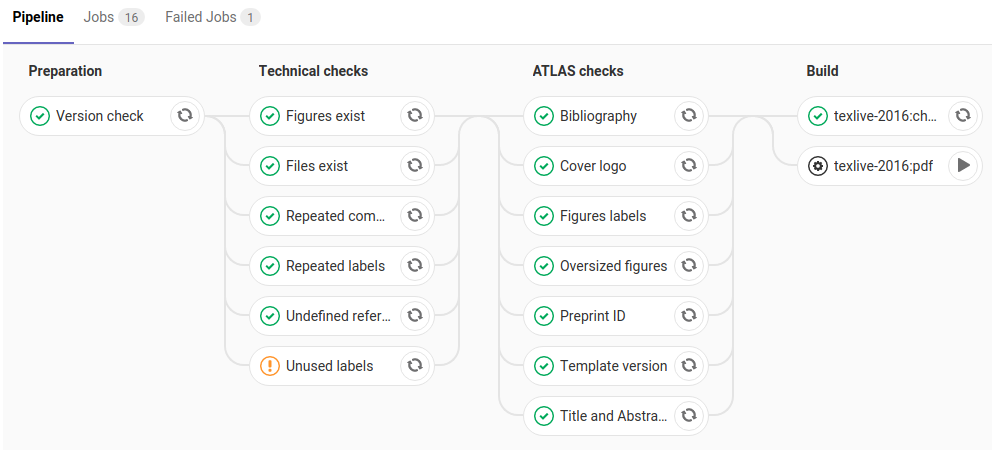
\includegraphics[width=0.9\textwidth]{edit-pipe.png}
  \caption{Screenshot of \epipe.}
  \label{fig:edit-pipe}
\end{figure}

\begin{table}
  \centering
  \begin{tabular}{l|c|c}
    \toprule
    \textbf{Document type} & \textbf{Preliminary label} & \textbf{Interl label} \\
    \midrule
    PAPER	& Not allowed	& Not allowed \\\midrule
    BOOK &	Not allowed	& Not allowed \\\midrule
    CONF &	Allowed	& Not allowed \\\midrule
    PUB &	Allowed	& Not allowed \\\midrule
    NOTE &	Allowed	& Allowed \\\bottomrule
  \end{tabular}
  \caption{Labels allowed and not allowed in figures depending on the document type.}
  \label{tab:labels-files}
\end{table}
